% use paper, or submit
% use 11 pt (preferred), 12 pt, or 10 pt only

\documentclass[letterpaper, preprint, paper,11pt]{AAS}	% for preprint proceedings
%\documentclass[letterpaper, paper,11pt]{AAS}		% for final proceedings (20-page limit)
%\documentclass[letterpaper, paper,12pt]{AAS}		% for final proceedings (20-page limit)
%\documentclass[letterpaper, paper,10pt]{AAS}		% for final proceedings (20-page limit)
%\documentclass[letterpaper, submit]{AAS}			% to submit to JAS

\usepackage{amssymb}

\usepackage{bm}
\usepackage{amsmath}
\usepackage{subfigure}
%\usepackage[notref,notcite]{showkeys}  % use this to temporarily show labels
\usepackage[colorlinks=true, pdfstartview=FitV, linkcolor=black, citecolor= black, urlcolor= black]{hyperref}
\usepackage{overcite}
\usepackage{footnpag}			      	% make footnote symbols restart on each page
\usepackage{graphicx}
\usepackage[textwidth=18mm,textsize=footnotesize,tickmarkheight=4pt]{todonotes}
\renewcommand{\eqref}[1]{Eq.~(\ref{#1})}

\newcommand{\md}{MD}
\newcommand{\ts}{s}
\newcommand{\tf}{f}


\PaperNumber{XX-XXX}



\begin{document}

\title{Warning Time Optimisation of Low-Thrust Satellite Collision Avoidance via Differential Algebra }

\author{Frank de Veld\thanks{PhD Student, Department of Mathematics, INRIA/Universit\'e C\^ote d'Azur, 06000, Nice, France.},  
Roberto Armellin\thanks{Professor, Te Pu\=naha \=Atea Auckland Space Institute, The University of Auckland, 1010, Auckland, New Zealand}, Zeno Pavanello\thanks{??} }



\maketitle{} 		


\begin{abstract}
The increasing density of space debris necessitates frequent and efficient collision avoidance maneuvers (CAMs) for operational satellites. This work presents a novel methodology that determines the latest possible thrust initiation time of low-thrust CAMs with differential algebra, offering a balance in accuracy and computational efficiency making it suitable for on-board CAM optimisation. In particular, this work dynamically tracks the time of maximum conjunction danger as a function of the control input, and leverages this tracking to find the latest possible time at which a thrust arc can be initiated while safely avoiding a collision between an operational satellite and a non-cooperative object.
\end{abstract}








\section{Introduction}

Recently, the increasing presence of space debris in Earth-centered orbits has posed significant challenges for satellite operators. As space debris objects orbit the Earth uncontrollably, they can pose a threat of collision to actively operated satellites nearby. Due to the high relative speeds involved, any collision would cause significant damage to satellites. Satellites are therefore forced to perform collision avoidance manoeuvres (CAMs) to stay clear of a collision when a close encounter is predicted to occur.

Many satellites in crowded operational orbits primarily use low-thrust propulsion systems, such as ion engines, Hall Effect thrusters and electrospray propulsion. Although these systems are more efficient than high-thrust propulsion, they reduce manoeuvrability, and manoeuvres such as CAMs can require minutes or even hours of thrust arcs. This limitation makes it important to start a satellite thrust arc adequately in advance, and can make optimisation of these arcs a complex task.

Existing literature primarily focuses on optimising CAM thrust arcs for fuel consumption or $\Delta$v, typically resulting in early maneuvers. However, operational constraints often favor delaying CAMs as long as possible to leverage updated tracking data and reduce unnecessary maneuvers. The danger of a satellite-debris conjunction is often assessed in terms of the probability of collision (PoC), a metric based on the propagated position uncertainty distribution. This uncertainty is regularly updated through ongoing tracking of the debris object. More recent tracking data results in less positional uncertainty and therefore a more accurate assessment of conjunction danger and whether a CAM is needed or not. 

Therefore, this work focuses on optimising the warning time for the CAM, that is, investigating the latest possible moment in time at which a thrust arc can be initiated to safely avoid a collision (i.e., decreasing the PoC to a safe threshold). Not only is this kind of optimisation pertinent to collision alerts which are received very late, but it can also be used to investigate whether there is enough time left to wait for the next batch of debris tracking data to arrive and re-assess whether a CAM is necessary. Earlier, this problem has been investigated in our prior work from an optimal control standpoint \cite{dell2024characterization}. While rigorous, it can be complicated to include for example inequality constraints in this methodology
% If the latest possible time to start the CAM thrust arc occurs before this data arrives

Existing techniques for low-thrust CAM optimisation often rely on numerical integration, which can be computationally intensive, or analytical approximations, which may sacrifice accuracy. For example, Pavanello et al. explored recursive polynomial methods for designing fast low-thrust collision avoidance manoeuvres, emphasising the potential for continuous optimisation of thrust profiles \cite{pavanello2024}. Mahfouz et al. investigated fuel-optimal formation reconfiguration using unidirectional low-thrust propulsion systems, focusing on minimising fuel consumption through advanced trajectory optimisation techniques, which is a different objective than optimising warning time \cite{Mahfouz2025}. Paduraru et al. applied reinforcement learning to optimise low-thrust CAMs, demonstrating improvements in computational efficiency compared to traditional methods, but the computational demands may be prohibitive for on-board implementation \cite{paduraru2024}.

Despite these advances in CAM optimisation, limitations such as the high computational cost of numerical methods and the potential inaccuracies of analytical approximations persist. Differential Algebra (DA) offers a promising alternative by efficiently propagating state and uncertainty information through Taylor series expansions. This allows for fast and accurate computation of the state and its derivatives, crucial for collision avoidance in dynamic and uncertain orbital environments, and they are flexible regarding the inclusion of operational constraints. This work leverages DA to address these challenges, aiming to enhance both the precision and computational feasibility of low-thrust CAM optimisation, specifically the optimisation of warning time.

Pavanello et al. have previously investigated low-thrust CAM optimisation, enabling efficient computation of the uncertainty distribution of objects involved in a conjunction at any point in time. Their approach integrates seamlessly with advanced higher-order methods, such as second-order cone programming, to address the non-convex nature of CAM optimisation problems \cite{pavanello2024b}. Building on the DA-based uncertainty propagation methods developed by Pavanello et al., this work introduces a novel approach by treating the time of maximum danger as a variable rather than a fixed parameter, as is commonly done. By allowing the time of maximum danger to vary, this methodology provides greater flexibility and accuracy and enables manoeuvres to shift the time of maximum danger further into the future.


In recent years, more attention has been paid to actively removing dangerous debris objects from orbit, but this work is still in its first steps. With more and more active satellites in orbit and enhanced debris tracking capabilities increasing the number of debris objects tracked, the number of CAMs required for safe space operations will only increase in coming years. Industry is working towards automated on-board collision avoidance, for which robust and efficient CAM optimisation algorithms are required. The DA methodology introduced in this work can contribute significantly to this goal.


This work is organised into a number of sections. First, the dynamics of the system and the close approach are presented, with the second part applying the DA techniques to the problem. Results about the performance of the methodology are then presented, as well as some strengths and weaknesses of the approach, followed by a conclusion.

\section{Problem dynamics}

We consider a controlled primary satellite described by a state 
\[
x_p = \begin{bmatrix} r_p \\ v_p \end{bmatrix} \in \mathbb{R}^6, \quad r_p \in \mathbb{R}^3 \text{ its position, and } v_p \in \mathbb{R}^3 \text{ its velocity},
\]
having a close encounter with a secondary uncontrolled satellite
\[
x_s = \begin{bmatrix} r_s \\ v_s \end{bmatrix} \in \mathbb{R}^6, \quad r_s \in \mathbb{R}^3, \quad v_s \in \mathbb{R}^3.
\]
The dynamics of the two objects are given by:
\begin{align}\label{eq:StateDynamics}
	\frac{d x_p}{dt} &= F(x_p) + \epsilon G(x_p) u, \\
	\frac{d x_s}{dt} &= F(x_s),
\end{align}
where \( F(\cdot): \mathbb{R}^6 \rightarrow \mathbb{R}^6 \) in \eqref{eq:StateDynamics} denotes the drift, representing uncontrolled motion of the objects. \( F(\cdot) \) can include any dynamics, though in this work we limit the drift to two-body acceleration only. \( \epsilon \in \mathbb{R} \) denotes the maximum acceleration due to thrust, \( G(x_p): \mathbb{R}^6 \rightarrow \mathbb{R}^{6 \times 3} \) the influence of control on the dynamics, and \( u \in \mathcal{U} \subset \mathbb{R}^3 \) the normalised control, representing thrust acceleration. In this work, we express $u$ in RSW-components, meaning that $G(\cdot)$ involves a frame transformation from RSW to ECI (in which the state vector is expressed).


Our primary focus is on the \textit{time of maximum danger}, denoted by $t_{MD}$, at which the chosen danger metric is evaluated. In this work, we consider only \textit{short encounters}, meaning that the danger metric is only assessed at $t_{MD}$, rather than in an entire time interval. It is therefore sufficient to design a collision avoidance manoeuvre which changes the danger metric to safety at $t_{MD}$ only. 

To evaluate the safety of a close approach, three commonly used metrics are often considered. The first is the Euclidean distance, defined as 
\begin{equation}\label{eq:EucDis}
d_E = \| r_p - r_s \|,
\end{equation}

where \( r_p \) and \( r_s \) are the positions of the primary and secondary satellites, respectively, and \( \| \cdot \| \) denotes the Euclidean norm. 

The second commonly used metric is the Mahalanobis distance, which accounts for the shape and orientation of the positional uncertainty ellipsoids and is defined as
\begin{equation}\label{eq:MD}
	d_M = \sqrt{(r_p - r_s)^\top \Sigma^{-1} (r_p - r_s)}.
\end{equation}

The Mahalanobis distance provides a normalised measure of separation that incorporates both the relative distance and the positional uncertainties. These metrics offer complementary perspectives on collision risk and are used depending on the context and precision required.

The third metric is the probability-of-collision formula, which estimates the likelihood of collision based on the relative position and positional uncertainty. For two satellites with Gaussian-distributed positional uncertainties, the probability of collision can be expressed as
\begin{equation}\label{eq:PoC}
d_{PoC} = \frac{R^2}{2 \pi \sqrt{\det(\Sigma)}} \exp\left( -\frac{1}{2} d_M^2 \right),
\end{equation}

making use of the definition of the Mahalanobis distance $d_M$, where \( \Sigma = \Sigma_p + \Sigma_s \) is the combined covariance matrix, with \( \Sigma_p \) and \( \Sigma_s \) representing the covariance matrices of the primary and secondary satellites, respectively. $R$ is the combined hard-body radius representing the physical size of the objects.

From now on, $d_{(\cdot)}$ represents the danger of distance metric of a conjunction, without specifying the exact metric choice.

\subsection{Optimisation Problem}

Regardless of the danger metric used, the goal of a Collision Avoidance Maneuver (CAM) is to reduce this metric to a safe threshold at \( t_{MD} \), thereby ensuring that the threshold is not exceeded for any \( t \) during short encounters. The objective is to maximise the time available before initiating the CAM, which is equivalent to minimising $-t_s$, where $t_s$ is the (negative) start time of the manoeuvre:

\begin{equation}\label{eq:OriginalProblem}
	\begin{aligned}
		&\min_{||u|| \leq 1} -t_{\ts} \quad \text{subject to:} \\ % Use \ts instead of t_s if defined
		&\quad \left\{ % Add the left brace here, indented with \quad
		\begin{aligned} % Start nested aligned for the two lines inside the brace
			&\frac{dx_p}{dt} = F(x) + \varepsilon G(x) \, u, \quad \forall t \in [t_0, t_{\md}], \\[10pt] % Keep original spacing
			&u \in \mathcal{U} \in \mathbb{R}^3, \quad \forall t \in [t_0, t_{\md}],
		\end{aligned} % End nested aligned
		\right. \\ % Add invisible right delimiter and end the line for the outer aligned
		% Add desired vertical space AFTER the braced group if needed, e.g., \\[10pt] above
		&\quad x_p(t_{\ts}) = x_{p,t_{\ts}}, \\[5pt]
		&\quad d_{(\cdot)}(t_{\tf}) = \sigma_{(\cdot)}, \\[5pt]
		&\quad t_{\tf} = t_{\md}(t_{\tf}), % Use \tf, \md if defined
	\end{aligned}
\end{equation}
where \( t_s \) and \( t_f \) denote the start and end times of the problem (and the CAM thrust arc), respectively. Here, \( t_{MD} \) is nominally assumed to be zero, meaning that \( t_s \)  is negative, and minimising \( -t_s \) corresponds to maximising the thrust initiation time. The initial state \( x_p(t_s) \) is determined by propagating the natural drift of the primary satellite backward in time from the current state. The parameter \( \sigma \) represents the safety threshold, which depends on the specific danger metric employed. Operationally, values like $\sigma_{E} = 1$ km as a minimum Euclidean distance or $\sigma_{PoC} = 10^{-4}$ as a maximum PoC are often used \cite{symonds2014operational}. Finally, the constraint \( t_f = t_{MD}(t_f) \) ensures that the final time of the optimisation problem coincides with the \textit{actual} time of maximum danger, which may vary due to the control input. The thrust arc is then ensured to cover the entire time interval $[t_s, t_{MD}]$, with $t_{MD}$ variable under control.

To account for the variation of $t_{MD}$ with the control input, we leverage an approximation based on the Euclidean distance metric. At the point of closest approach, the relative position and velocity vectors are orthogonal:
\begin{equation}\label{eq:TrackTCA}
	(r_p(t_{MD}) - r_s(t_{MD})) \cdot (v_p(t_{MD}) - v_s(t_{MD})) = 0,
\end{equation}
where the relative position vector and the relative velocity vector are orthogonal at the moment of geometric closest approach. While this orthogonality condition holds strictly for the Euclidean distance, we use it as a first-order approximation for $t_{MD}$ when using the PoC or Mahalanobis distance, recognising that these metrics also incorporate uncertainty information, as the geometric closest approach often aligns closely with the time of maximum danger. For small uncertainties, these metrics are dominated by the relative distance, validating the use of orthogonality as a first-order approximation.

\section{Differential Algebra Approach}

In order to use differential algebra effectively in the context of the optimisation problem shown in \eqref{eq:OriginalProblem}, it is convenient to discretise the time grid between $t^{alert}$ (the time at which a dangerous conjunction in the future is noticed) and $\bar{t}_{MD}$ (the nominal time of maximum danger), where $t^{alert} < t_s < t_{MD}$. Obtained is a discretised time grid $t_0, t_1, ..., t_N$ of $N$ intervals, where $t_0 = t^{alert}$ and $t_N = \bar{t}_{MD}$.  

We consider \( r_p(t_{N-1}) \) and \( v_p(t_{N-1}) \), the state of the primary satellite at time \( t_{N-1} \), as:
\begin{align}
	r_p(t_{N-1}) &= \bar{r}_p(t_{N-1}) + \delta r_p(t_{N-1}), \\
	v_p(t_{N-1}) &= \bar{v}_p(t_{N-1}) + \delta v_p(t_{N-1}),
\end{align}
that is to say, they are vectors described by the sum of their nominal state (\( \bar{r}_p(t_{N-1}) \) and \( \bar{v}_p(t_{N-1}) \)) and possible perturbations (\( \delta r_p(t_{N-1}) \) and \( \delta v_p(t_{N-1}) \)) caused by control \( u \). The state of the secondary object is unchanged: 
\[
r_s(t_{N-1}) = \bar{r}_s(t_{N-1}), \quad 
v_s(t_{N-1}) = \bar{v}_s(t_{N-1}),
\]
as the control \( u \) does not act on the secondary object.


We consider a possible thrust duration from $t_0 = t^{alert}$ to $t_N = \bar{t}_{MD}$, assuming that the optimal time of starting thrust $t_s$ is within this range. To facilitate the DA implementation, we introduce a time transformation:
\begin{equation}\label{eq:Tau}
	\tau = \frac{t}{T} 	
\end{equation} 
, where $T = \bar{t}_{MD} - t_0$, leading to $\frac{d}{dt} = \frac{d}{d \tau} \frac{1}{T}$. Note that $T$ can vary under the influence of control, as the time of maximum danger $t_{MD}$ is strongly dependent on the orbit of the primary satellite. We can therefore write 
\begin{equation}
	T(t_{N-1}) = \bar{t}_{MD} + \delta t = t_{MD}
\end{equation}
for some perturbation $\delta t$. For simplicity, we initially assume a constant thrust profile  $u([t_{N-1}, \bar{t}_{MD} + \delta t]) = 0 + \delta u([t_{N-1} , \bar{t}_{MD} + \delta t])$ in RSW components in within each time interval: a zero nominal thrust profile and a thrust perturbation $\delta u$.

The state at $t_{MD} + \delta t$ is computed by propagating the perturbed state at $t_{N-1}$ using a Taylor series expansion (obtained via DA) that incorporates the effects of the control perturbations ($\delta u$) and the time perturbation ($\delta t$): \eqref{eq:Taylors} maps the perturbed state of the primary satellite at time $t_{N-1}$ to the nominal time of maximum danger $\bar{t}_{MD}$, where $\mathcal{T}(\cdot)$ represents the Taylor series expansion obtained from the DA-based propagation. This approach allows us to express the system's behaviour as Taylor polynomials in terms of perturbations $\delta r_p$, $\delta v_p$, $\delta u$ and $\delta t$. 

\begin{equation}\label{eq:Taylors}
	\begin{cases}
		r_p(\bar{t}_{MD} + \delta t) = \mathcal{T}(\delta r_p(t_{N-1}), \delta v_p(t_{N-1}), \delta u([t_{N-1}, \bar{t}_{MD} + \delta t]), \delta t) \\
		v_p(\bar{t}_{MD} + \delta t) = \mathcal{T}(\delta r_p(t_{N-1}), \delta v_p(t_{N-1}), \delta u([t_{N-1}, \bar{t}_{MD} + \delta t]), \delta t) \\
		r_s(\bar{t}_{MD} + \delta t) = \mathcal{T}(\delta t) \\
		v_s(\bar{t}_{MD} + \delta t) = \mathcal{T}(\delta t) \\
		r_{\text{rel}}(\bar{t}_{MD}+ \delta t) = \mathcal{T}(\delta r_p(t_{N-1}), \delta v_p(t_{N-1}), \delta u([t_{N-1}, \bar{t}_{MD} + \delta t]), \delta t) \\
		v_{\text{rel}}(\bar{t}_{MD}+ \delta t) = \mathcal{T}(\delta r_p(t_{N-1}), \delta v_p(t_{N-1}), \delta u([t_{N-1} , \bar{t}_{MD} + \delta t]), \delta t) \\
		\Delta \tau(\bar{t}_{MD}+ \delta t) = \mathcal{T}(\delta r_p(t_{N-1}), \delta v_p(t_{N-1}), \delta u([t_{N-1}, \bar{t}_{MD} + \delta t]), \delta t) \\
	\end{cases}
\end{equation}
Here, $r_{\text{rel}} = r_p - r_s$ and $v_{\text{rel}}  = v_p - v_s$ are defined as the relative position and velocity respectively, in the case of \eqref{eq:Taylors} at time $\bar{t}_{MD} + \delta t$, and $\Delta \tau$ the change in thrust duration as a result of the aforementioned perturbations. Note that $\delta r_p$ and $\delta v_p$ cover perturbations at $t_{N-1}$, $\delta u$ covers a perturbation in the interval $[t_{N-1}, \bar{t}_{MD} + \delta t]$ and $\delta t$ covers a perturbation at the end of the time interval $[t_{N-1}, \bar{t}_{MD}]$. The state of the secondary satellite is unaffected by control, and the Taylor polynomials describing the state in \eqref{eq:Taylors} are therefore only dependent on $\delta t$.

To ensure the control-induced perturbations accurately mitigate collision risk, $\delta t$ must satisfy the closest approach condition, where the relative position and velocity vectors are orthogonal.
The time perturbation $\delta t$ is determined by enforcing the orthogonality condition (\eqref{eq:ResolvingDeltaT}) at perturbed time $\bar{t}_{MD} + \delta t$, linking perturbations at $t_{N-1}$ to the geometric closest approach:
%We can resolve $\delta t$ by mandating that a geometric closest approach is tracked at $\bar{t}_{MD} + \delta t$. If we use the Euclidean norm as a danger metric, the nominal time of maximum danger $\bar{t}_{MD}$ already denotes a geometric closest approach, meaning that $\Delta r \cdot \Delta v = 0$ at $\bar{t}_{MD}$ and $\bar{t}_{MD} + \delta t$. We obtain

\begin{equation}\label{eq:ResolvingDeltaT}
	\delta t = \delta t_{CA} = \mathcal{T}(\delta r(t_{N-1}), \delta v(t_{N-1}), \delta u([t_{N-1}, \bar{t}_{CA} + \delta t]))
\end{equation}

The orthogonality condition $r_{\text{rel}}\cdot v_{\text{rel}} =0$ at $t_{MD}$ ensures that the derived $\delta t$ corresponds to the time when the relative distance between the objects is minimal. This guarantees the perturbations are accurately aligned with the dynamics of the conjunction. Resolving $\delta t$ ensures that all evaluations at $\bar{t}_{MD} + \delta t$ track the moment of maximum danger.

Next, the danger metric at $\bar{t}_{MD} + \delta t$ (tracking $t_{MD}$) can be approximated by a Taylor polynomial like in \eqref{eq:Taylors}. Note that all danger metrics described in \eqref{eq:EucDis}, \eqref{eq:PoC} and \eqref{eq:MD} are primarily dependent on $r_{\text{rel}}$. We therefore also have 

\begin{equation}\label{eq:DMTaylor}
		d_{(\cdot)}(\bar{t}_{MD}+ \delta t) = \mathcal{T}(\delta r_p(t_{N-1}), \delta v_p(t_{N-1}), \delta u([t_{N-1}, \bar{t}_{MD} + \delta t]), \delta t)
\end{equation}

To determine the optimal control perturbation $\delta$u, we expand the danger metric $d_{(\cdot)}(\bar{t}_{MD} + \delta t)$ around the nominal value:
\begin{equation}\label{eq:DMExpansion}
	d_{(\cdot)}(\bar{t}_{MD} + \delta t) = d_{(\cdot)}(\bar{t}_{MD}) + \frac{\partial d_{(\cdot)}}{\partial \delta u} \delta u([t_{N-1},  \bar{t}_{MD} + \delta t]) + \mathcal{O}(||\delta u||^2)
\end{equation}

In low-thrust propulsion scenarios, the limited thrust magnitude ($\epsilon << 1$) necessitates precise targeting of the danger metric's rate of change to achieve optimal collision avoidance. To maximise the rate of change of the danger metric, the control perturbation  $\delta u$,  is chosen to be aligned with the gradient:

\begin{equation}\label{eq:Control}
	\delta u([t_{N-1}, \bar{t}_{MD} + \delta t]) = \epsilon \frac{ \frac{\partial d_{(\cdot)}}{\partial \delta u}}{|| \frac{\partial d_{(\cdot)}}{\partial \delta u}||}
\end{equation}

\eqref{eq:Control} can be substituted in \eqref{eq:DMTaylor}, together with $\delta r_p(t_{N-1}) = \delta v_p(t_{N-1}) = 0$ to investigate the effect of $\delta u([t_{N-1}, \bar{t}_{MD} + \delta t])$ on $d_{(\cdot)}(\bar{t}_{MD} + \delta t)$. There are now two cases possible:

\begin{itemize}
	\item If $d_{(\cdot)}(\bar{t}_{MD} + \delta t)$ exceeds the safety threshold $\sigma_{(\cdot)}$, we refine the solution within the interval $t_{N-1}, t_{N}$ to obtain a more precise value of $t_s$
	\item $d_{(\cdot)}(\bar{t}_{MD} + \delta t)$ has not yet reached the safety threshold $\sigma_{(\cdot)}$. In that case, we consider the time interval $[t_{N-2}, t_{N-1}]$ and obtain the following system: 
	\begin{equation}\label{eq:TaylorsBack2}
		\begin{cases}
			r_p(t_{N-1}) = \mathcal{T}(\delta r_p(t_{N-2}), \delta v_p(t_{N-2}), \delta u([t_{N-2}, t_{N-1}]), \delta t) \\
			v_p(t_{N-1}) = \mathcal{T}(\delta r_p(t_{N-2}), \delta v_p(t_{N-2}), \delta u([t_{N-2}, t_{N-1}]), \delta t) \\
			r_s(t_{N-1}) = \mathcal{T}(\delta t) \\
			v_s(t_{N-1}) = \mathcal{T}(\delta t) \\
		\end{cases}
	\end{equation}
	Root-finding can be used to obtain $\delta t$ again, ensuring a tracking of the closest approach, and $r_p(t_{N-1})$, $v_p(t_{N-1})$, $r_s(t_{N-1})$ and $v_s(t_{N-1})$ can be substituted in \eqref{eq:DMTaylor}, together with \eqref{eq:Control}, obtaining $\delta u([t_{N-2}, t_{N-1}])$. The same process can now be repeated for previous time steps.
\end{itemize}

A backward sweep is therefore performed over the time intervals $[t_{N - 1}, t_N + \delta t ]$, $[t_{N-2}, t_{N-1}]$, ...., $[t_0, t_1]$ until the safety threshold $\sigma_{(\cdot)}$ is reached, depending on the exact danger metric, and $t_s$ can be found accordingly.


The idea of the methodology is sketched out in \autoref{fig:DiagramOfGeometry}, with a nominal trajectory in blue along discretised time steps $t_{j}$, $j \in [0,N]$
\begin{figure}[!h]
	\centering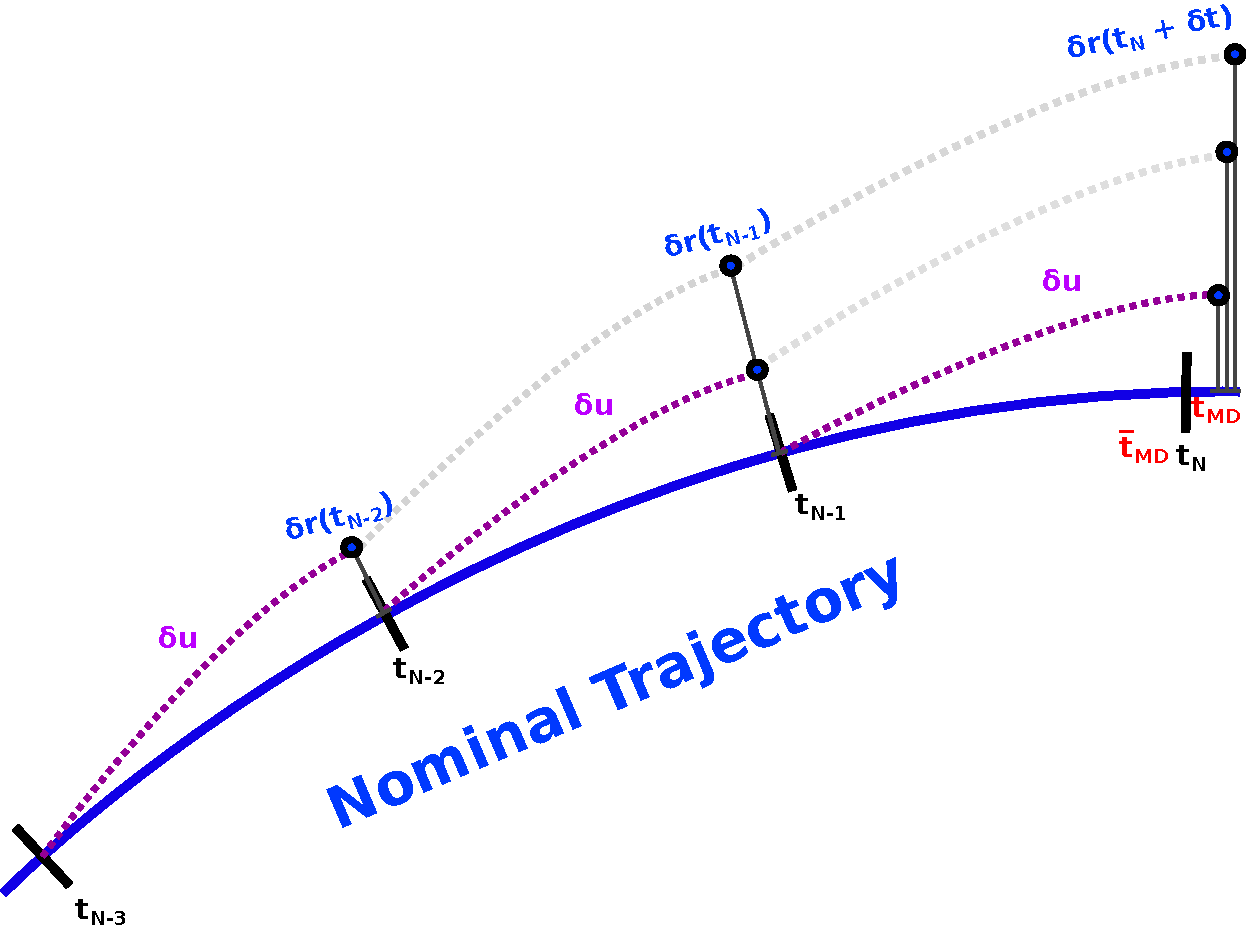
\includegraphics[width=12 cm]{Figures/BackwardSweep.pdf}
	\caption{Illustration of the backward sweep procedure using Differential Algebra. The nominal trajectory is shown in blue, with discrete time steps. Perturbations in position ($\delta$r), velocity ($\delta$v), and control ($\delta$u) are used to iteratively refine the manoeuvre start time ($t_s$).}
	\label{fig:DiagramOfGeometry}
\end{figure}
Starting at the time interval $[t_{N-1},t_N]$, where $t_N = \bar{t}_{MD}$ the nominal time of maximum danger, the position deviation $\delta r(t_N + \delta t)$ is tracked, depending on $\delta r_p(t_{N-1})$, $\delta v_p(t_{N-1})$ (not explicitly shown), $\delta u$ in the time interval $[t_{N-1},t_N + \delta t]$, and $\delta t$ itself. $\delta t$ can be found through polynomial inversion with \eqref{eq:ResolvingDeltaT} and $\delta u$ through rate-of-change maximisation of $d_{(\cdot)}$ in \eqref{eq:Control}. In this first time interval, $\delta r_p(t_{N-1})$ and $\delta v_p(t_{N-1})$ are zero, enabling computation of $\delta r_p(t_N + \delta t)$; the lower one of the right three black dots in \autoref{fig:DiagramOfGeometry}. Going back one time interval to $[t_{N-2},t_{N-1}]$ and performing the same method, $\delta r_p(t_{N-1})$ and  $\delta v_p(t_{N-1})$ are obtained. Their non-zero values are substituted in the Taylor polynomial for $\delta r_p(t_N + \delta t)$, which now shifts to the second of the right three black dots in \autoref{fig:DiagramOfGeometry} under the influence of control in the time interval $[t_{N-2},t_{N-1}]$. The same can be done for the time interval $[t_{N-3},t_{N-2}]$, shown by  the upper of the three black dots in \autoref{fig:DiagramOfGeometry}. 


\section{Applications}
While the proposed methodology is valid for a wide range of satellite conjunctions, the geometry of the conjunction can play a significant role, not only in the control profile $u(t)$, but also in the methodology accuracy. As mentioned, the control profile requires discretisation in the DA methodology described in this work and is assumed to have constant components in the time intervals. Therefore, when the optimal control profile changes rapidly, the discretised control might be less accurate. Additionally, the combined covariance of the primary and secondary objects changes over time for non-circular orbits, increasing near the periapsis and decreasing near the apsis. 

In this section, the algorithm is applied to a representative case study of a typical ISS-like orbit, having close to zero eccentricity in Low-Earth Orbit. Simulation parameters are shown in \autoref{tb:Parameters}.
%one/two representative test cases:
%\begin{itemize}
%	\item An ISS-like orbit with zero eccentricity in Low-Earth Orbit
%	\item (Possibly?) A GTO-like eccentric orbit with high eccentricity and altitude ranging from 500 to 40000 km
%\end{itemize}


\begin{table}[!h]
	\centering
	\caption{Simulation parameters}
	\label{tb:Parameters}
	\begin{tabular}{|l|c|}
		\hline
		\textbf{Parameter}             & \textbf{Case Study (ISS-like)} \\ \hline % & \textbf{Case Study 2 (GTO-like)} \\ \hline
		Semi-major axis, $a$ (km)      & 6780                            \\% & 24582                              \\ \hline
		Eccentricity, $e$              & $10^{-3}$    \\%                         & 0.73                              \\ \hline
		Inclination, $i$ (deg)         & 51.6         \\%                    & 27                              \\ \hline
		RAAN, $\Omega$ (deg)           & 0            \\%                 & 0                              \\ \hline
		Argument of Perigee, $\omega$ (deg) & 0       \\%                  & 270                              \\ \hline
		True Anomaly, $\nu$ at $\bar{t}_{MD}$ (deg) & 30     \\%                 & 90                              \\ \hline
		Thrust Magnitude, $\epsilon$ (m/s\(^2\)) & $1.0 \cdot  10^{-4}$         \\%          &                              \\ \hline
		Gravitational Parameter, $\mu$ (m\(^3\)/s\(^2\)) & $3.986 \cdot 10^{14}$       \\%   &                              \\ \hline
		Number of Nodes, $N$           & 50                             \\%&                              \\ \hline
		Alert Time, $t^{alert}$ (s)   & -1800                              \\%&                              \\ \hline
		Nominal miss distance, $d_{E}$ (m)    & 200                             \\%&                              \\ \hline
		Safe miss distance, $\sigma_{E}$ (m)   & 1000                              \\%&                              \\ \hline
		Nominal standard deviation, $\sigma_{x}$ (m)    &    100                        \\% &                              \\ \hline
		Nominal covariance, $\rho_{xy}$ (m$^2$)    &            0.4                \\%&                              \\ \hline
		Nominal standard deviation, $\sigma_{y}$ (m)    &  75                        \\%   &                              \\ \hline
		Safe PoC, $\sigma_{PoC}$     &  $10^{-5}$                           \\%&                              \\ % \hline
		Safe Mahalanobis distance, $\sigma_{M}$ (-)    &  3                        \\   \hline % &                              \\ \hline
	\end{tabular}
\end{table}

In the Results section, the control profiles $u(t)$ are investigated for the case study and the different danger metrics $d_{E}$, $d_{PoC}$ and $d_{M}$, and the change in danger metrics over time is also shown.
%The number of nodes $N$ and the true anomaly at $\bar{t}_{MD}$ are varied to highlight their influence.

\section{Results}\label{sec:Results}

The discretised control profile $u(t)$ of the first case study with an ISS-like orbit is shown in \autoref{fig:Case1Control}, for three different distance metrics:

\begin{figure}[!h]
	\centering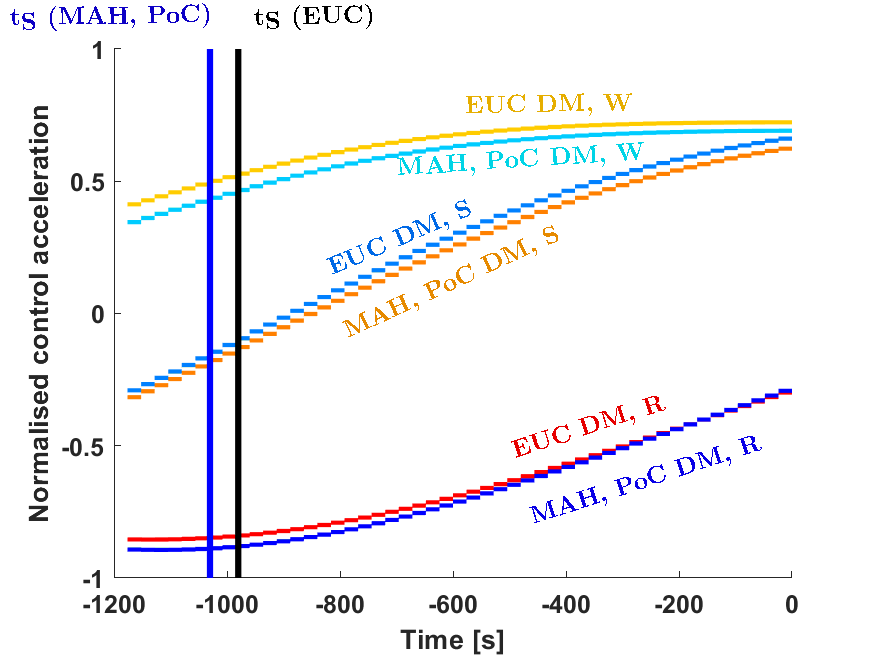
\includegraphics[width=12 cm]{Figures/ControlCaseStudy1.pdf}
	\caption{The control profile (radial, along-track and cross-track components) over time for the Euclidean, Mahalanobis and PoC distance metrics, and the latest time to initiate thrust}
	\label{fig:Case1Control}
\end{figure}

The discrete nature of the control in \autoref{fig:Case1Control} is clear, as the control components are constant within the discrete time intervals. The Mahalanobis and PoC-based control profiles are nearly identical, as both depend heavily on the covariance matrix $\Sigma$. They differ slightly from the control profile based on the Euclidean distance danger metric, but not significantly. Vertical lines in \autoref{fig:Case1Control} indicate the maximum $t_s$ values for each distance metric. These values are not the same for the three danger metrics, as $d_M$ and $d_{PoC}$ depend to a large extent on the combined covariance $\Sigma$, while $d_E$ does not.


Additionally, the change of the Euclidean distance danger metric throughout the backward sweep is shown in \autoref{fig:Case1DangerMetric}.

\begin{figure}[!h]
	\centering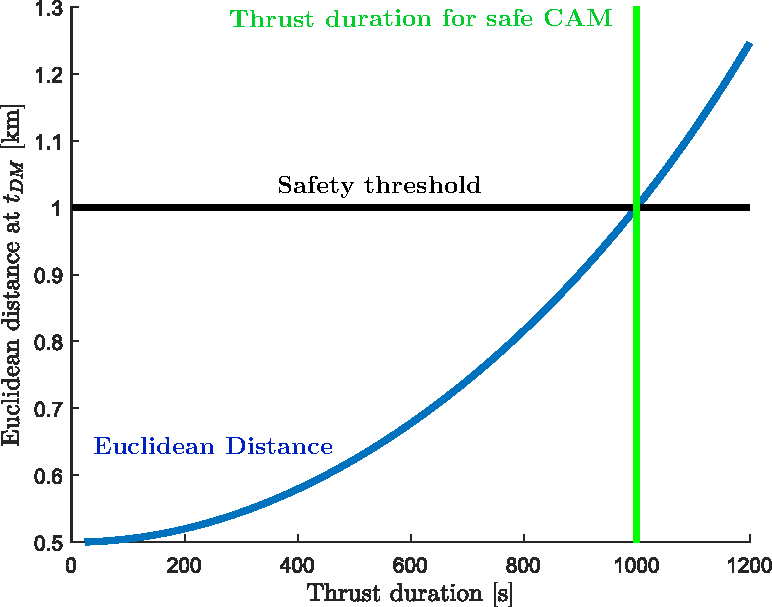
\includegraphics[width=12 cm]{Figures/DMEAAS.pdf}
	\caption{The Euclidean distance metric for various thrust durations}
	\label{fig:Case1DangerMetric}
\end{figure}

The thrust duration is shown in \autoref{fig:Case1DangerMetric}, rather than the time $t$ itself, coinciding with $t_{MD} - t_s$. $t_{MD}$ varies with time in principle, but the change from its nominal value is less than a second and not visible in \autoref{fig:Case1Control} and \autoref{fig:Case1DangerMetric}. Since the control is unconstrained in direction, the Euclidean distance metric is continuously increasing with thrust until the safe threshold is reached. 

\section{Conclusion and discussion}

The introduced DA methodology provides several advantages for low-thrust CAM optimisation. First, the control profile minimising \(-t_s\) is quickly determined using a first-order approximation. Given the small thrust magnitudes involved, this first-order solution is often sufficiently accurate. If needed, it can be refined to second-order accuracy by extending the Taylor expansion of the danger metric \(d_{(\cdot)}\). Furthermore, the methodology is flexible, allowing the use of various danger metrics beyond the three mentioned in this work. Additionally, operational constraints, such as restricted thrust intervals or directional limitations, can be seamlessly integrated into the DA framework.

% The combined covariance matrix \(\Sigma\) can also be expanded as a Taylor polynomial to enhance accuracy, if necessary -> Removed because this is not trivial

One of the methodology's key strengths is its explicit tracking of \( t_{MD} \), the time of maximum danger. This is achieved through polynomial inversion of the \(\delta t\) term, not only in the time interval \([t_{N-1}, \bar{t}_{MD} + \delta t]\) but also in earlier intervals. During the backward sweep, \( t_{MD} \) is accurately updated through the Taylor polynomial representing $r_{\text{rel}}(\bar{t}_{MD} + \delta t)$, ensuring that the danger metric \(d_{(\cdot)}\) is evaluated at the correct time. However, the control profile \(u_{t_{N-1} \to \bar{t}_{MD} + \delta t}\) is not recalculated in earlier intervals. In other words, once \(\delta t\) is resolved for \([t_{N-1}, \bar{t}_{MD} + \delta t]\), the thrust continues uninterrupted until the recalculated \( t_{MD} \). Earlier control profiles \( u_{t_{i-1} \to t_i} \) (\(i = 1, 2, \dots, N-1\)) adjust \( t_{MD} \) as \(\delta t\) evolves, but they do not retroactively modify the control in subsequent intervals.

Despite these advantages, the methodology has some limitations. The control profile \( u \) must be discretised over time, with constant components in each time interval. Choosing an appropriate discretisation number \( N \) can be challenging, and modelling errors may be introduced if the true optimal control profile \( u^* \) (found e.g. using optimal control theory) varies rapidly within an interval. Additionally, the methodology heavily depends on two key assumptions: (1) that the time of maximum danger coincides with the geometric closest approach, and (2) that thrust magnitudes remain small relative to the natural dynamics. As a result, this approach is unsuitable for impulsive CAMs or long encounters with small \(||v_{\text{rel}}||\) values between the primary and secondary.


\section{Acknowledgments}
The authors would like to express their gratitude to the developers of the DACE library for C++ for providing software that enabled efficient differential algebra computations utilised in this work. The authors also extend their appreciation to Thales Alenia Space for their sponsorship of a portion of the PhD program under which this research was conducted. Furthermore, the authors acknowledge the support of Université Côte d’Azur for funding a research stay in Auckland, New Zealand, which greatly contributed to the progress of this work.





%The introduced DA methodology has many advantages for application in low-thrust CAM optimisation. The control minimising $-t_s$ is quickly found in first-order approximation. Due to the small thrust magnitudes involved in the problem, first-order control is often sufficiently accurate, and can relatively easily be replaced by second order control following the Taylor expansion of $d_{(\cdot)}$. Many different danger metrics $d_{(\cdot)}$ can be used for the CAM optimisation problem apart from the three mentioned in this work, and the combined covariance matrix $\Sigma$ can be expanded as a Taylor polynomial as well for increased accuracy. Additionally, operational constraints, like time intervals of forbidden thrust and constraints in thrust direction can easily be incorporated into the DA methodology.
%
%The methodology offers an extra layer of accuracy in CAM optimisation through the explicit tracking of $t_{MD}$, the time of maximum danger. This is done through polynomial inversion of the $\delta t$ term, not only in the time interval $[t_{N-1}, \bar{t}_{MD} + \delta t]$, $\delta t$, but also for time intervals before. In earlier time intervals, $t_{MD}$ is still accurately tracked through the Taylor polynomial denoting $\Delta r(\bar{t}_{MD} + \delta t)$, ensuring evaluation of $d_{(\cdot)}$ at the correct time. However, $u_{t_{N-1} \rightarrow \bar{t}_{MD} + \delta t}$ is not re-evaluated further in the backward sweep. That is, for the time interval $[t_{N-1}, \bar{t}_{MD} + \delta t]$, $\delta t$ is resolved and the thrust continues until $t_{MD}  = \bar{t}_{MD} + \delta t$, the recalculated time of maximum danger as a result of the control $u_{t_{N-1} \rightarrow \bar{t}_{MD} + \delta t}$. However, control in earlier intervals $u_{t_{i-1} \rightarrow t_{i}}$ for $i = 1, 2, ..., N-1$ also adjusts $t_{MD}$ as $\delta t$ changes to track $t_{MD}$ accurately, but $u_{t_{N-1} \rightarrow \bar{t}_{MD} + \delta t}$ is in principle not recalculated
%
%A downside of the methodology is that the control profile $u$ needs to be discretised in time and needs to have constant components in the discretised time intervals. Not only can it be challenging to choose an appropriate discretisation number $N$, inaccuracies can occur when the true optimal control profile $u^*$ changes rapidly. Apart from that, the DA methodology of this work heavily depends on the approximation that the time of maximum danger coincides with geometric closest approach and that thrust magnitudes are small compared to the natural dynamics. The methodology therefore cannot easily be applied to impulsive CAMs and long encounters with a small $\Delta v$ between the primary and the secondary.

%The algorithm consists of the following steps:
%
%\subsection{Initial State Propagation}
%The primary satellite (controllable) and secondary object (non-controllable) are propagated to the nominal time of closest approach ($\bar{t}_{CA}$) based on their respective nominal trajectories. The nominal state for the primary is given by $(\vec{r}_{p_0}(t), \vec{v}_{p_0}(t))$, while the secondary follows $(\vec{r}_{s_0}(t), \vec{v}_{s_0}(t))$. 
%
%\subsection{Time Discretisation}
%The interval between the alert time ($t^{alert}$) and $\bar{t}_{CA}$ is divided into $N$ steps: $t_0 = t^{alert}$ and $t_N = \bar{t}_{CA}$. The algorithm processes the grid in reverse, starting at $t_{N-1}$.
%
%\subsection{State Perturbation Representation}
%At $t_{N-1}$, the primary's position and velocity are expressed as perturbed states:
%\begin{align*}
%	\vec{r}_p(t_{N-1}) &= \vec{r}_{p_0}(t_{N-1}) + \delta \vec{r}(t_{N-1}), \\
%	\vec{v}_p(t_{N-1}) &= \vec{v}_{p_0}(t_{N-1}) + \delta \vec{v}(t_{N-1}),
%\end{align*}
%where $\delta \vec{r}$ and $\delta \vec{v}$ are DA variables. The secondary state remains nominal:
%\begin{align*}
%	\vec{r}_s(t_{N-1}) &= \vec{r}_{s_0}(t_{N-1}), \\
%	\vec{v}_s(t_{N-1}) &= \vec{v}_{s_0}(t_{N-1}).
%\end{align*}
%
%\subsection{Thrust Duration and Scaling}
%The thrust duration $T$ is expressed as $T = \bar{t}_{CA} + \delta t - t_0$, where $\delta t$ is treated as a DA variable. A time-scaling transformation is applied: $\tau = t / T$, yielding $\frac{d}{dt} = \frac{1}{T} \frac{d}{d\tau}$.

%\subsection{Conjunction Metric Formulation}
%The conjunction metric, such as the Square Mahalanobis Distance (SMD), is expressed as a Taylor polynomial:
%\begin{align*}
%	\text{SMD}(\bar{t}_{CA} + \delta t) = \mathcal{T}(\delta \vec{r}(t_{N-1}), \delta \vec{v}(t_{N-1}), \delta \vec{u}(t_{N-1} \to \bar{t}_{CA} + \delta t), \delta t).
%\end{align*}
%This metric incorporates the position and velocity differences projected onto the B-plane and weighted by the combined covariance matrix $P$.
%
%\subsection{Optimisation of Thrust Control}
%To optimise the thrust control $\delta \vec{u}$, the first-order expansion of the SMD is considered:
%\begin{align*}
%	\text{SMD} = \overline{\text{SMD}} + \frac{\partial \text{SMD}}{\partial \delta \vec{u}} \delta \vec{u}(t_{N-1} \to \bar{t}_{CA} + \delta t) + \mathcal{O}(||\delta \vec{u}||^2),
%\end{align*}
%where $\overline{\text{SMD}}$ is the nominal value without control. The optimal thrust direction is computed as:
%\begin{align*}
%	\delta \vec{u} = \epsilon \frac{\frac{\partial \text{SMD}}{\partial \delta \vec{u}}}{|| \frac{\partial \text{SMD}}{\partial \delta \vec{u}} ||},
%\end{align*}
%with $\epsilon$ being the thrust magnitude.
%
%\subsection{Backward Sweep}
%If the SMD under the influence of thrust does not exceed the threshold, the algorithm steps back to $t_{N-2}$ and repeats the optimisation, propagating the perturbed states:
%\begin{align*}
%	\delta \vec{r}_p(t_{N-1}) &= \mathcal{T}(\delta \vec{r}(t_{N-2}), \delta \vec{v}(t_{N-2}), \delta \vec{u}(t_{N-2} \to t_{N-1}), \delta t) - \vec{r}_{p_0}(t_{N-1}), \\
%	\delta \vec{v}_p(t_{N-1}) &= \mathcal{T}(\delta \vec{r}(t_{N-2}), \delta \vec{v}(t_{N-2}), \delta \vec{u}(t_{N-2} \to t_{N-1}), \delta t) - \vec{v}_{p_0}(t_{N-1}).
%\end{align*}
%The process continues until the SMD surpasses the threshold or operational constraints are reached.


% The close encounter is characterised by a time of maximum danger $t_d$
% (Part about the actual optimisation technique, differential algebra, and why this was chosen)
% debris not removed, detection capabilities increased -> CAMs will stay relevant on-board computation, quick, easy

%The American Astronautical Society (AAS) publishes bound sets of printed conference proceedings for personal, institutional, and library usage. The availability of hardcopy enhances the longevity of your work and elevates the importance of your conference contribution to professionals through archival publication. To preserve the consistency and quality of the proceedings, all authors adhere to the latest version of AAS conference proceedings format.


%This document is intended to serve as a visual and instructional guide, and as a \LaTeX\ document template, for the AAS conference proceedings format. This template provides the basic font sizes, styles, and margins required by the publisher's formatting instructions.   There are also styles for centered equations, figure and table captions, section and sub-section headings, footnote text, \emph{etc}. This template provides samples of their usage.  To use this document as a template, simply copy and change its contents with your own information while maintaining the required predefined style, rather than starting anew. Since this is not a tutorial on how to use \LaTeX\, refer to \LaTeX\ manuals for more information.


%Your manuscript should include a paper number, a title, an author listing, an abstract, an introductory section, one or more sections containing the main body of the manuscript, a concluding summary section, and a reference or bibliography section. You may also include a section on notation, an acknowledgements section, and appendices, as illustrated in the sequel. You should \emph{not} include a leading cover sheet. Author affiliation shall appear on the first page, added as a footnote to the last name of each the author. If a distributional release statement or copyright notice is required by your sponsor, this is added as a footnote to the title of the manuscript, appearing on the first page only. Page numbers should be centered halfway between the lower margin and the bottom edge of the page (\emph{i.e.}, approximately 0.75 inches from the bottom). Copy should be single space with double space between paragraphs, with the first line of each paragraph indented 0.2 inches.

%The recommended sans-serif font for paper number, title, and author listing is \emph{Arial}, or, \emph{Helvetica}. The title font and paper-number font should be the same: 14-point sans-serif, centered, and bold. The author-listing font should be 12-point sans-serif, centered, and bold. The recommended serif font for body text, headings, \emph{etc}., is \emph{Times} or \emph{Times New Roman} at 10-12 point, 11 point preferred. The captions for figures and tables are bold 10-point serif font. The endnote reference text and footnote text is 9-point serif font. The right-hand margin of body text should be justified; if not, it should be fairly even nevertheless. All text and text background shall remain uncolored (black on white). These conventions should be automatically implemented in this \LaTeX\ template when the predefined styles of this template are used.

%The body text of this template is based on the preferred font size of 11 points. To change this to 12-point size, increase the font size at the top of the \LaTeX\ template by uncommenting the appropriate {\tt documentclass[]\{\}} line. For very long manuscripts, a 10-point font may be used to keep the manuscript within the publisher's limit of twenty (20) physical pages.


%\section{This is a Sample of a General Section Heading}
%Numbering of section headings and paragraphs should be avoided. Major section headings are majuscule, bold, flush (aligned) left, and use the same style san-serif font as the body text. Widow and orphan lines should also be avoided; more than one line of a paragraph should appear at the end or beginning of a page, not one line by itself. A heading should not appear at the bottom of a page without at least two lines of text. Equations, figures, and tables must be sequentially numbered with no repeated numbers or gaps. Excessive white space --- such as large gaps before, between, and after text and figures --- should be minimal and eliminated where possible.





%\subsection{This Is a Sample of a Secondary (Sub-Section) Heading}
%Secondary, or sub-section, headings are title case (miniscule lettering with the first letter of major words majuscule), flush left, and bold. Secondary headings use the same serif font style as the body text and, like section headings, should not be numbered. Tertiary headings should be avoided, but if necessary, they are run-in, italic, and end in a period, as illustrated with the next six (6) paragraphs.
%\begin{equation}
%	\label{eq:ab}
%	a = b^{2}
%\end{equation}
%
%\subsubsection{Equations.} 
%Equations are centered with the equation number flush to the right. In the text, these equations should be referenced by name as Eq.~\eqref{eq:ab} or Equation~\eqref{eq:ab} (\emph{e.g}., not eq. 1, (1), or \emph{Equation 1}). To improve readability, scalar variable names such as $a$ and $b^{2}$ are usually italicized when appearing in text and equations.\footnote{A section on mathematical notation is provided in the sequel.}
%


%\subsubsection{Abbreviations.} 
%When abbreviations for units of measure are used, lower case without periods is preferred in most instances; \emph{e.g}. ft, yd, sec, ft/sec, \emph{etc}., but in. for inch.
%
%
%
%
%\begin{figure}[htb]
%	\centering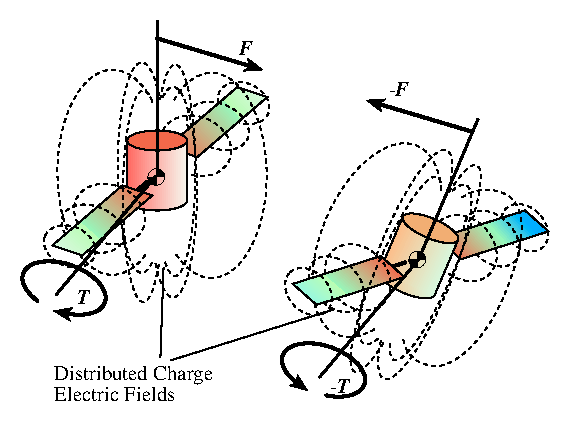
\includegraphics[width=3.5in]{Figures/test}
%	\caption{Illustration Caption Goes Here}
%	\label{fig:xxx}
%\end{figure}

%\subsubsection{Figures.}   
%Illustrations are referenced by name and without formatting embellishments, such as Figure~\ref{fig:xxx}, Figure 2, \emph{etc}., or, Figures 3 and 4 (\emph{e.g}., not figure (1), Fig. 1, \underline{Figure 1}, \emph{Figure 1}, \emph{etc}.). Each illustration should have a caption unless it is a mere sketch. Single-phrase captions are usually in title case; they are bold 10-point serif font and centered below the figure as shown in Figure~\ref{fig:xxx}. An explanatory caption of several sentences is permissible. Ideally, every illustration should be legibly sized -- usually about one-half or one-quarter page -- and appear in the text just before it is called out or mentioned. Alternatively, it is also permissible to place all figures together at the end of the text as a separate appendix; however, these two conventions should not be mixed. All figures and callouts should remain clearly legible after reduction. All illustrations appear as black and white in the final printing, although colors are retained in the electronic (CD-ROM) version.

%
%\subsubsection{Graphic Formats.} 
%The highest quality formats are Encapsulated PostScript (EPS) and PDF vector-graphic formats. These formats are recommended for all illustrations, unless they create document files that are excessively large. Specifically, you should change the graphic format or compress the image resolution whenever an illustrated page takes more than two seconds to render onscreen, or, whenever the total manuscript file size starts to approach 5 Mb. Photographs, illustrations that use heavy toner or ink (such as bar graphs), and figures without text callouts, may be suitably displayed with picture formats such as BMP, GIF, JPEG, PNG, TIFF, \emph{etc}. Line drawings, plots, and callouts on illustrations, should not use picture formats that do not provide sharp reproduction. All graphical content must be embedded when creating a PDF document, especially any fonts used within the illustration. Note that the Windows Metafile Format (WMF) is sometimes problematic and should be avoided.
%
%
%\subsubsection{References and Citations.} 
%The citation of bibliographical endnote references is indicated in the text by superscripted Arabic numerals, preferably at the end of a sentence.\cite{doe2005, style1959}   If this citation causes confusion in mathematics, or if a superscript is inappropriate for other reasons, this may be alternately expressed as (Reference~\citenum{doe2005}) or (see References~\citenum{doe2005} and \citenum{style1959}), (\emph{e.g}., not [1], Ref. (1), \emph{etc}.). While there is no singly prescribed format for every bibliographical endnote, references should be consistent in form. Citations should be sufficient to allow the reader to precisely find the information being cited, and should include specific pages, editions, and printing numbers where necessary. URL citations are discouraged, especially when an archival source for the same information is available. If a URL citation is required, it should appear completely and as a footnote instead of a bibliographical reference.\footnote{\url{http://www.univelt.com/FAQ.html\#SUBMISSION}}  The citation of private communication is especially discouraged, but if required it should be cited as a footnote and include the date, professional affiliation, and location of the person cited.\footnote{Gangster, Maurice (1999), personal correspondence of March 21st. Sr. Consultant, Space Cowboy Associates, Inc., Colorado Springs, CO.}  


%
%\begin{table}[htbp]
%	\fontsize{10}{10}\selectfont
%    \caption{A Caption Goes Here}
%   \label{tab:label}
%        \centering 
%   \begin{tabular}{c | r | r } % Column formatting, 
%      \hline 
%      Animal    & Description & Price (\$)\\
%      \hline 
%      Gnat      & per gram & 13.65 \\
%                & each     &  0.01 \\
%      Gnu       & stuffed  & 92.50 \\
%      Emu       & stuffed  & 33.33 \\
%      Armadillo & frozen   &  8.99 \\
%      \hline
%   \end{tabular}
%\end{table}
%
%\emph{Tables.} 
%Tables are referred to by name in the text as Table~\ref{tab:label}, or, Tables 2 and 3 (\emph{e.g}., not table 1, Tbl. 1, or \emph{Table 1}). The title is centered above the table, as shown in Table 1. The font size inside tables should be no larger than the body text, but may be adjusted down to 9-point if necessary (10-point serif font is considered nominal). Note that table units are in parentheses. Only the minimum number of table lines needed for clarity is desired. Ideally, every table should appear within the text just before it is called out, but, it is also permissible to place all tables together at the end of the text as a separate appendix. If so, these two conventions should not be mixed.
%
%Equations, figures, and tables must be sequentially numbered with no repeated numbers or gaps. Each figure and table shall be called out in the text; gratuitous figures and tables that are not called out should be eliminated. Intermediate equations may be numbered without being called out.




%\section{Manuscript Submission}
%The Portable Document Format (PDF) is the preferred format for electronic submissions.\footnote{By contributing your manuscript for proceedings publication, you necessarily extend any copyrights to the AAS and its designated publisher, to allow the AAS to publish your manuscript content in all the forms that it wishes.}
% The page size should be 8.5 inches by 11 inches exactly. You should use ``press-quality'' or ``high-quality'' software settings to create your PDF file; these settings tend to keep the PDF file true to the original manuscript layout, and automatically embed the correct fonts, \emph{etc}. Otherwise, settings such as ``Embed All Fonts'', \emph{etc}., should be selected as available. The use of internal hyperlinks within the electronic file is not encouraged because hyperlinks may not be supported in the final version of the electronic proceedings.
%
%\subsection{Journal Submission}
%If you wish to submit this manuscript to the \emph{Journal of Astronautical Sciences}, it must be re-formatted into a double-spaced format. This can be done easily with this template. At the top of the document, there are two (2) types document class statements ({\tt paper} and {\tt submit}).  The first type is the one to use for a conference paper.  The second type , which is commented out, can be used to reformat the paper for the JAS journal submission.


%\section{Conclusion}
%TBD



%
%\section{Notation}
%\begin{tabular}{r l}
%	$a$ & a real number \\
%	$b$ &  the square root of $a$ \\
%\end{tabular} \\
%
%If extensive use of mathematical symbols requires a table of notation, that table may appear here. Where the first mathematical symbol is introduced, a footnote should direct the attention of the reader to this table.\footnote{The footnote symbols are a standard sequence: $\ast$, $\dagger$, $\ddag$, \emph{etc}. This sequence of footnote symbols should restart with each new page.}  The notation table should be simple and reasonably consistent with the standards of modern technical journals, as illustrated above. The notation table does not need its own caption like an ordinary table, since the section heading serves this purpose. The notation section is optional.





%\appendix
%\section*{Appendix: Title here}
%Each appendix is its own section with its own section heading. The title of each appendix section is preceded by ``APPENDIX: '' as illustrated above, or ``APPENDIX A: '', ``APPENDIX B: '', \emph{etc}., when multiple appendixes are necessary. Appendices are optional and normally go after references; however, appendices may go ahead of the references section whenever the word processor forces superscripted endnotes to the very end of the document. The contents of each appendix must be called out at least once in the body of the manuscript.
%
%
%\subsection*{Miscellaneous Physical Dimensions}
%The page size shall be the American standard of 8.5 inches by 11 inches (216 mm x 279 mm). Margins are as follows: Top -- 0.75 inch (19 mm); Bottom -- 1.5 inches (38 mm); Left -- 1.25 inches (32 mm); Right -- 1.25 inch (32 mm). The title of the manuscript starts one inch (25.4 mm) below the top margin. Column width is 6 inches (152.5 mm) and column length is 8.75 inches (222.5 mm). The abstract is 4.5 inches (114 mm) in width, centered, justified, 10 point normal (serif) font.


\bibliographystyle{AAS_publication}   % Number the references.
\bibliography{references}   % Use references.bib to resolve the labels.



\end{document}
